\section{Ti\textit{k}Z package}

\begin{quote}
    2020-05-01: first update
\end{quote}

\subsection{Examples}

\begin{enumerate}

\item drawing a square
    
\begin{lstlisting}[language=Tex]
\begin{tikzpicture}
    \draw (0,0) -- (0,2) -- (2,2) -- (2,0) -- (0,0);
    % end in the start to form a cycle
    \draw (0,0) -- (0,2) -- (2,2) -- (2,0) -- cycle;
    % use the rectangle keyword to simplify
    \draw (0,0) rectangle (4,4);
\end{tikzpicture}
\end{lstlisting}

\begin{tikzpicture}
    %\draw (0,0) -- (0,2) -- (2,2) -- (2,0) -- (0,0);
    %\draw (0,0) -- (0,2) -- (2,2) -- (2,0) -- cycle;
    \draw (0,0) rectangle (2,2);
\end{tikzpicture}

\item drawing a parabola

\begin{lstlisting}[language=Tex]
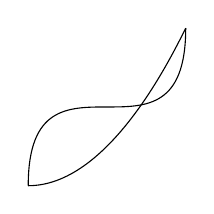
\begin{tikzpicture}
     \draw (0,0) parabola (2,2);
     % add control points
    \draw (0,0) .. controls (0,2) and (2,0) .. (2,2);
\end{tikzpicture}
\end{lstlisting}

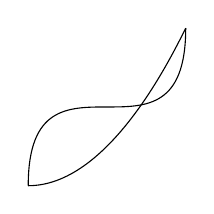
\begin{tikzpicture}
    \draw (0,0) parabola (2,2);
    % add control points
    \draw (0,0) .. controls (0,2) and (2,0) .. (2,2);
\end{tikzpicture}

\item draw a circle

\begin{lstlisting}[language=Tex]
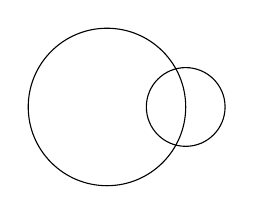
\begin{tikzpicture}
     % center and radius
    \draw (1,1) circle (1cm);
    \draw (2,1) circle (0.5cm);
\end{tikzpicture}
\end{lstlisting}

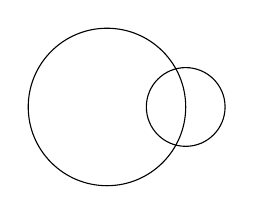
\begin{tikzpicture}
    \draw (1,1) circle (1cm);
    \draw (2,1) circle (0.5cm);
\end{tikzpicture}

    
\end{enumerate}


\subsection{Useful links}

\begin{enumerate}

    \item \href{https://mirror.foobar.to/CTAN/graphics/pgf/base/doc/pgfmanual.pdf}{The TikZ and PGF Packages}
    
        Manual for version 3.1.8b, December 27, 2020
    
\end{enumerate}